\documentclass{report}
\usepackage[utf8]{inputenc}
\usepackage[a4paper, right=2.5cm, left=2.5cm, top=2cm, bottom=2cm]{geometry}
\usepackage{graphicx}
\usepackage[french]{babel}

\usepackage{lmodern}
\usepackage[T1]{fontenc}
\usepackage{amssymb}
\usepackage{amsmath}
\usepackage{amsthm}
\usepackage{fancyhdr}
\usepackage{hyperref}
\usepackage{float}
\usepackage{microtype}
\setlength{\emergencystretch}{3em}
\usepackage{titling}
\usepackage{subcaption}
\usepackage{booktabs}
\usepackage{tabularx}
\usepackage[french]{cleveref}

\renewcommand*\familydefault{\sfdefault}
\hypersetup{
    colorlinks=true,
    linkcolor=blue,
    filecolor=magenta,
    urlcolor=cyan,
    pdftitle={Rapport RDFIA},
    }
\urlstyle{same}

\title{Reconnaissance des formes pour l'analyse et l'interprétation d'images}

\author{Jean-Léo Serrano, Théophile Lahaussois, Théo Fontaine}
\date{Année 2026 -- 2027}

\fancyhead{}
\fancyhead[L]{RDFIA}\fancyhead[R]{2026 -- 2027}
\pagestyle{fancy}
\thispagestyle{plain}

\begin{document}

\begin{titlepage}
    \centering

    \vspace*{\fill}
    \Huge \thetitle \par
    \vspace{2mm}
    \Large \textbf{Travaux pratiques d'apprentissage profond} \par
    \vspace{2mm}

    \Large \theauthor \par
    \vspace{2mm}
    \large \thedate \par

    \vfill

    \large Sorbonne-Université

\end{titlepage}

\tableofcontents
\newpage

\chapter*{Introduction}
\addcontentsline{toc}{chapter}{Introduction}

\noindent
L'apprentissage profond en vision par ordinateur s'est développé à travers trois grands axes :
\begin{enumerate}
    \item \textbf{Les réseaux entièrement connectés (MLP)} se basent sur la rétropropagation du gradient qui utilise la formule de la dérivation en chaîne. Ces réseaux permettent d'apprendre des frontières de décision qui ne sont pas linéaires sans nécessiter l'astuce du noyau des SVM classiques, mais ne tiennent pas compte de la topologie 2D des images.
    \item \textbf{Les réseaux de neurones convolutifs (CNN)} sont construits en partageant les poids des convolutions, ainsi que la connectivité locale. Les CNN utilisent les biais inductifs de localité spatiale et d'équivariance par translation (complétée par l'invariance locale qu'apporte le \textit{pooling}), ce qui leur a permis de devenir la référence sur des jeux d'images tels que MNIST et CIFAR-10~\cite{lecun1998, krizhevsky2012}.
    \item \textbf{Les Vision Transformers (ViT)} sont inspirés du traitement du langage naturel. Les ViT n'utilisent pas de biais de localité lorsqu'ils traitent l'image comme une séquence de patchs connectés entre eux par un mécanisme d'auto-attention globale~\cite{dosovitskiy2021}.
\end{enumerate}

\noindent
Ce rapport répond à chacune des questions dans les trois travaux pratiques (ab, cd, cde).

\chapter{Introduction aux réseaux de neurones (1-ab)}

Cette première partie porte sur l'étude d'un perceptron multicouche à une couche cachée appliqué à la classification binaire sur le jeu de données non linéaire \textit{Circles}, suivie de son extension au jeu de données MNIST.

\section{Fondements théoriques}
\subsection{Jeu de données supervisé}

\paragraph{1. $\bigstar$ À quoi servent les ensembles d'entraînement, de validation et de test ?}
L'ensemble d'\textbf{entraînement} sert à apprendre les paramètres du modèle (poids et biais) grâce à la descente du gradient. L'ensemble de \textbf{validation} sert à choisir les hyperparamètres comme la taille de la couche cachée, le pas d'apprentissage, le nombre d'époques et la régularisation, et à détecter le surapprentissage, sur des données que l'optimisation n'a pas vues. L'ensemble de \textbf{test} n'est utilisé qu'une seule fois à la fin pour estimer sans biais l'erreur de généralisation du modèle final. Utiliser l'ensemble de test pour régler les hyperparamètres revient à apprendre sur cet ensemble, ce qui rend son estimation trop optimiste.

\paragraph{2. Quelle est l'influence du nombre d'exemples $N$ ?}
Plus la valeur de $N$ est grande, plus la perte moyenne sur l'entraînement s'approche du risque réel, ce qui signifie en conséquence que le modèle généralise mieux. À l'inverse, une petite valeur de $N$ rend le modèle beaucoup plus sensible au bruit des exemples et limite sa capacité de prédiction. La valeur de $N$ augmente aussi le coût d'une époque et les gains s'atténuent lorsque $N$ devient grand. Enfin, la taille des ensembles de validation et de test a une influence sur la précision des estimations. Avec 200 exemples de test sur \textit{Circles}, un exemple vaut à peu près $0.5$ point de précision.

\subsection{Architecture du réseau (\textit{forward})}
\paragraph{3. Pourquoi est-il important d'ajouter des fonctions d'activation entre les transformations linéaires ?}
Une composition de transformations affines reste affine, \emph{e.g.} $W_2(W_1 x + b_1) + b_2 = (W_2 W_1) x + (W_2 b_1 + b_2)$. Sans aucune activation non linéaire, un réseau de profondeur quelconque ne devient pas plus expressif qu'une unique couche linéaire, et ne peut donc produire que des frontières de décision linéaires. Pour \textit{Circles}, ce choix est insuffisant. Les activations non linéaires rendent le réseau capable d'approcher n'importe quelle fonction continue. Elles permettent aussi de contraindre l'intervalle des sorties ($[-1, 1]$ pour $\tanh$ par exemple).

\paragraph{4. $\bigstar$ Quelles sont les tailles $n_x$, $n_h$, $n_y$ dans la figure 1 ? En pratique, comment ces tailles sont-elles choisies ?}
Dans la figure 1, nous avons $n_x = 2$ (entrées $x_1, x_2$), $n_h = 4$ (neurones $h_1$ à $h_4$) et $n_y = 2$ (sorties $\hat{y}_1$ et $\hat{y}_2$). Le réseau compte donc $4 \times 2 + 4 = 12$ paramètres dans la couche cachée et $2 \times 4 + 2 = 10$ dans la couche de sortie (les poids $w^h_{ij}$ et $w^y_{ij}$ de la figure, plus les biais). En pratique, il faut poser les valeurs de $n_x$ et $n_y$ selon le problème : $n_x$ est la dimension des caractéristiques ($2$ pour \textit{Circles}, $784$ pour MNIST) et $n_y$ est le nombre de classes ($2$, puis $10$). $n_h$ est un hyperparamètre qui règle la capacité du réseau. Lorsqu'il est trop petit, le modèle sous-apprend. Lorsqu'il est trop grand, le modèle risque de surapprendre. Il faut alors les choisir sur l'ensemble de validation. Nous avons utilisé $n_h = 10$ sur \textit{Circles} et $n_h = 100$ sur MNIST.

\paragraph{5. Que représentent les vecteurs $\hat{y}$ et $y$ ? Quelle est la différence entre ces deux quantités ?}
$y$ est la vraie valeur, il s'agit d'un vecteur \textit{one-hot} qui vaut 1 sur la vraie classe et 0 ailleurs. $\hat{y}$ est la prédiction du réseau et correspond à une distribution de probabilité sur les classes ($\hat{y}_i \in [0, 1]$, $\sum_i \hat{y}_i = 1$), où $\hat{y}_i$ est la probabilité de correspondre à la classe $i$. La différence entre ces deux valeurs est mesurée par la fonction de perte et correspond à ce que l'algorithme d'apprentissage cherche à réduire. La classe prédite est $\arg\max_i \hat{y}_i$.

\paragraph{6. Pourquoi utiliser une fonction Softmax comme fonction d'activation de sortie ?}
Softmax transforme les scores réels $\tilde{y}$ en une distribution de probabilité. Il s'agit de sorties positives et dont la somme vaut 1. Softmax est une version dérivable de l'$\arg\max$. Son fonctionnement repose sur le fait que la classe de score maximal reçoit la plus grande probabilité sans pour autant annuler le gradient des autres. La fonction softmax peut être utilisée avec l'entropie croisée, qui compare deux distributions. Le calcul du gradient de l'ensemble se simplifie en $\hat{y} - y$.

\paragraph{7. Écrire les équations mathématiques permettant d'effectuer la passe \textit{forward} du réseau, c'est-à-dire de produire successivement $\tilde{h}$, $h$, $\tilde{y}$ et $\hat{y}$ à partir de $x$.}
Pour une entrée $x \in \mathbb{R}^{n_x}$ :
\begin{gather*}
    \tilde{h} = W_h x + b_h, \qquad
    h = \tanh(\tilde{h}), \qquad
    \tilde{y} = W_y h + b_y, \\
    \hat{y} = \mathrm{Softmax}(\tilde{y}), \ \text{soit} \ \hat{y}_i = \frac{e^{\tilde{y}_i}}{\sum_{j=1}^{n_y} e^{\tilde{y}_j}},
\end{gather*}
avec $W_h \in \mathbb{R}^{n_h \times n_x}$, $b_h \in \mathbb{R}^{n_h}$, $W_y \in \mathbb{R}^{n_y \times n_h}$ et $b_y \in \mathbb{R}^{n_y}$. La version par batch utilisée dans le code est donnée en section 2.1.

\subsection{Fonction de perte}
\paragraph{8. Pendant l'apprentissage, on cherche à minimiser la fonction de perte. Pour l'entropie croisée et l'erreur quadratique, comment les $\hat{y}_i$ doivent-ils varier pour faire diminuer la perte globale $\mathcal{L}$ ?}
\begin{itemizeFB}
\item\textbf{Entropie croisée} : $\ell = -\sum_i y_i \log \hat{y}_i = -\log \hat{y}_c$, où $c$ est la vraie classe. Seule la probabilité de la vraie classe est utilisée dans la formule finale : il faut augmenter $\hat{y}_c$ vers 1. Comme $\sum_i \hat{y}_i = 1$, les probabilités des autres classes diminuent vers 0. 
\item\textbf{Erreur quadratique} : $\ell = \sum_i (y_i - \hat{y}_i)^2$. Chaque sortie doit se rapprocher de sa cible. De ce fait, $\hat{y}_c$ doit augmenter vers 1 et chaque $\hat{y}_i$ ($i \neq c$) doit diminuer vers 0. Dans les deux cas, la perte est nulle lorsque $\hat{y} = y$.

\end{itemizeFB}

\paragraph{9. En quoi ces fonctions sont-elles mieux adaptées à la classification ou à la régression ?}
L'\textbf{entropie croisée} est la log-vraisemblance négative d'une loi catégorielle. La minimiser revient à estimer les probabilités des classes par maximum de vraisemblance, ce qui correspond exactement à un problème de classification. Elle pénalise de manière non bornée une prédiction à la fois confiante et fausse ($-\log \hat{y}_c \to +\infty$ quand $\hat{y}_c \to 0$). Combinée à une fonction Softmax, son gradient $\hat{y} - y$ reste élevé tant que l'erreur est importante. À l'inverse, l'\textbf{erreur quadratique} correspond à la log-vraisemblance négative d'un bruit gaussien. Elle convient à l'utilisation de la régression, c'est-à-dire à la prédiction de valeurs réelles continues, en pénalisant en même temps l'écart à la cible. Utilisée pour la classification après un Softmax, elle génère une pénalité bornée à 2 et des gradients qui s'annulent lorsque le Softmax sature, même en cas d'erreur, ce qui ralentit l'apprentissage.

\subsection{Algorithme d'optimisation}
\paragraph{10. Quels semblent être les avantages et les inconvénients des différentes variantes de descente de gradient (classique, stochastique par mini-batch, stochastique en ligne) ? Laquelle semble la plus raisonnable dans le cas général ?}
\begin{itemize}
	\item \textbf{Descente de gradient classique (batch complet)} : elle offre un gradient exact et une trajectoire stable. Cependant, elle n'effectue qu'une seule mise à jour par itération sur les données, son coût par itération est proportionnel à $N$ (ce qui la rend inapplicable aux grands jeux de données ou limitée par la mémoire GPU) et elle a tendance à rester bloquée dans des minima locaux ou des plateaux.
	\item \textbf{Descente stochastique en ligne (un seul exemple)} : elle permet des mises à jour très fréquentes et peu coûteuses, avec un bruit qui aide à s'extraire des mauvais minima. Cependant, ce gradient très bruité entraîne une convergence irrégulière qui oblige à réduire le pas d'apprentissage. L'absence de vectorisation la rend plutôt lente sur GPU.
	\item \textbf{Descente stochastique par mini-batch} : elle constitue un compromis entre les deux approches précédentes. L'écart-type du bruit du gradient décroît en $1/\sqrt{B}$. Les mises à jour restent nombreuses à chaque époque et le calcul sur un lot d'exemples est bien vectorisé sur GPU.
\end{itemize}
Le \textbf{mini-batch} s'impose donc comme le choix le plus pertinent dans le cas général. Nos expériences sur \textit{Circles} (\cref{fig-ab_bs}) l'illustrent. Pour un nombre d'époques égal, une taille de batch de 1 converge plus vite par époque mais la fonction de perte est très bruitée et le temps d'exécution est jusqu'à 9 fois plus long. Le batch complet n'a toujours pas convergé après 250 époques.

\paragraph{11. $\bigstar$ Quelle est l'influence du pas d'apprentissage (\textit{learning rate}) $\eta$ sur l'apprentissage ?}
Le pas d'apprentissage $\eta$ fixe l'amplitude de chaque mise à jour. S'il est trop petit, la convergence devient très lente. Par exemple, avec $\eta = 0.001$, la précision sur l'ensemble de test n'atteint que $60.7\%$ après 250 époques. S'il est trop grand, les mises à jour dépassent le minimum, ce qui fait osciller ou diverger la fonction de perte, ou provoque la saturation du réseau (les fonctions $\tanh$ et Softmax se bloquent respectivement à $\pm 1$ et $0/1$) et bloque l'apprentissage. Ainsi, pour $\eta = 2$, la précision en test atteint $63\%$ et se stabilise avec un écart-type de 18 points selon l'initialisation. Pour $\eta = 10$, la perte explose. Ainsi, augmenter $\eta$ permet d'accélérer la convergence mais a pour conséquence une trajectoire plus bruitée (\cref{fig-ab_lr}).

\paragraph{12. $\bigstar$ Comparer la complexité (en fonction du nombre de couches du réseau) du calcul des gradients de la perte par rapport aux paramètres, avec l'approche naïve et avec l'algorithme de rétropropagation.}
Pour un réseau à $L$ couches, le gradient par rapport aux paramètres de la couche $l$ s'exprime comme le produit de $L - l$ matrices jacobiennes, de la sortie jusqu'à la couche $l$. L'approche naïve recalcule ce produit indépendamment pour chaque couche, ce qui entraîne un coût de $\sum_{l=1}^{L} (L - l) = \mathcal{O}(L^2)$ produits de jacobiennes. À l'inverse, la rétropropagation calcule les gradients de la sortie vers l'entrée en réutilisant à chaque étape le gradient déjà obtenu pour la couche suivante selon la relation $\nabla_{l} = J_{l+1}^\top \nabla_{l+1}$. Chaque couche n'est ainsi parcourue qu'une seule fois, ce qui réduit la complexité à $\mathcal{O}(L)$ opérations, c'est-à-dire le même ordre de grandeur qu'une passe avant.

\paragraph{13. Quels critères l'architecture du réseau doit-elle respecter pour permettre une telle procédure d'optimisation ?}
Pour que la règle de dérivation en chaîne s'applique, toutes les opérations reliant les paramètres à la fonction de perte doivent être dérivables, au moins presque partout (comme c'est le cas pour ReLU ou le max-pooling). La perte elle-même doit être un scalaire. De plus, le réseau doit former un graphe orienté acyclique composé de fonctions élémentaires dont les dérivées locales sont connues. Un réseau récurrent doit ainsi être déroulé dans le temps pour satisfaire cette condition. En pratique, il est également indispensable que les gradients ne disparaissent pas ni explosent lors de leur propagation à travers les couches. C'est deux points influencent le choix des fonctions d'activation et la stratégie d'initialisation.

\paragraph{14. La fonction Softmax et la perte d'entropie croisée sont souvent utilisées ensemble et leur gradient est très simple. Montrer que la perte peut se simplifier en $\ell = -\sum_i y_i \tilde{y}_i + \log \big(\sum_i e^{\tilde{y}_i}\big)$.}
Avec $\hat{y}_i = e^{\tilde{y}_i} / \sum_j e^{\tilde{y}_j}$, on a $\log \hat{y}_i = \tilde{y}_i - \log \sum_j e^{\tilde{y}_j}$. Donc
\begin{equation*}
    \ell = -\sum_i y_i \log \hat{y}_i = -\sum_i y_i \tilde{y}_i + \Big(\sum_i y_i\Big) \log \sum_j e^{\tilde{y}_j} = -\sum_i y_i \tilde{y}_i + \log \sum_j e^{\tilde{y}_j},
\end{equation*}
puisque $\sum_i y_i = 1$ pour une cible \textit{one-hot}.

\paragraph{15. Écrire le gradient de la perte (entropie croisée) par rapport à la sortie intermédiaire $\tilde{y}$.}
En dérivant l'expression précédente :
\begin{equation*}
    \frac{\partial \ell}{\partial \tilde{y}_i} = -y_i + \frac{e^{\tilde{y}_i}}{\sum_j e^{\tilde{y}_j}} = \hat{y}_i - y_i
    \quad \Longrightarrow \quad
    \nabla_{\tilde{y}} \ell = \begin{pmatrix} \hat{y}_1 - y_1 \\ \vdots \\ \hat{y}_{n_y} - y_{n_y} \end{pmatrix} = \hat{y} - y.
\end{equation*}

\paragraph{16. À l'aide de la rétropropagation, écrire le gradient de la perte par rapport aux poids de la couche de sortie $\nabla_{W_y} \ell$, en utilisant $\nabla_{\tilde{y}} \ell$. Faire de même pour $\nabla_{b_y} \ell$.}
Comme $\tilde{y}_k = \sum_j W_{y,kj} h_j + b_{y,k}$, on a $\partial \tilde{y}_k / \partial W_{y,ij} = \delta_{ki}\, h_j$ (symbole de Kronecker : $\delta_{ki} = 1$ si $k = i$, $0$ sinon). D'où
\begin{equation*}
    \frac{\partial \ell}{\partial W_{y,ij}} = \sum_k \frac{\partial \ell}{\partial \tilde{y}_k} \frac{\partial \tilde{y}_k}{\partial W_{y,ij}} = (\nabla_{\tilde{y}} \ell)_i \, h_j
    \quad \Longrightarrow \quad
    \nabla_{W_y} \ell = \nabla_{\tilde{y}} \ell \; h^\top = (\hat{y} - y)\, h^\top \in \mathbb{R}^{n_y \times n_h}.
\end{equation*}
De même, $\partial \tilde{y}_k / \partial b_{y,i} = \delta_{ki}$, donc $\nabla_{b_y} \ell = \nabla_{\tilde{y}} \ell = \hat{y} - y$.

\paragraph{17. $\bigstar$ Calculer les autres gradients : $\nabla_{\tilde{h}} \ell$, $\nabla_{W_h} \ell$, $\nabla_{b_h} \ell$.}
On remonte d'abord vers $h$ : $\tilde{y}_k$ dépend de $h_j$ via $W_{y,kj}$, donc $\nabla_h \ell = W_y^\top \nabla_{\tilde{y}} \ell$. Comme $h_j = \tanh(\tilde{h}_j)$ et $\tanh' = 1 - \tanh^2$ :
\begin{equation*}
    \nabla_{\tilde{h}} \ell = \big(W_y^\top \nabla_{\tilde{y}} \ell\big) \odot (1 - h^2), \qquad
    \nabla_{W_h} \ell = \nabla_{\tilde{h}} \ell \; x^\top \in \mathbb{R}^{n_h \times n_x}, \qquad
    \nabla_{b_h} \ell = \nabla_{\tilde{h}} \ell,
\end{equation*}
où $\odot$ est le produit terme à terme et $h^2$ le carré terme à terme. Pour un mini-batch, la perte est la moyenne des pertes unitaires, donc les gradients des paramètres sont les moyennes de ces gradients sur le batch. C'est ce qu'implémente la fonction \texttt{backward} (section 2.1).

\section{Implémentation}
\subsection{\textit{Forward} et \textit{backward} manuels}

Cette sous-section répond aux questions 2 à 7 de la section 2.1 (fonctions \texttt{init\_params}, \texttt{forward}, \texttt{loss\_accuracy}, \texttt{backward}, \texttt{sgd} et boucle d'apprentissage).

\paragraph{Initialisation des paramètres (\texttt{init\_params}) :}
Pour $n_x$ entrées, $n_h$ neurones cachés et $n_y$ sorties, les poids sont tirés selon une loi normale centrée d'écart-type $0.3$ ($W_h \in \mathbb{R}^{n_h \times n_x}$, $W_y \in \mathbb{R}^{n_y \times n_h}$) et les biais sont initialisés à zéro ($b_h \in \mathbb{R}^{n_h \times 1}$, $b_y \in \mathbb{R}^{n_y \times 1}$).

\paragraph{Passe avant (\texttt{forward}) :}
Pour un batch $X \in \mathbb{R}^{B \times n_x}$, transposé en $X^\top \in \mathbb{R}^{n_x \times B}$ :
\begin{align}
    \tilde{h} &= W_h X^\top + b_h \quad \in \mathbb{R}^{n_h \times B}, \\
    h &= \tanh(\tilde{h}) \quad \in \mathbb{R}^{n_h \times B}, \\
    \tilde{y} &= W_y h + b_y \quad \in \mathbb{R}^{n_y \times B}, \\
    \hat{y}_{c, i} &= \frac{e^{\tilde{y}_{c, i} - \max_k \tilde{y}_{k, i}}}{\sum_{j=1}^{n_y} e^{\tilde{y}_{j, i} - \max_k \tilde{y}_{k, i}}}.
\end{align}
La soustraction du maximum par colonne dans le softmax évite un \textit{overflow}.

\paragraph{Perte et Précision (\texttt{loss\_accuracy}) :}
Pour les cibles \textit{one-hot} $Y \in \{0, 1\}^{B \times n_y}$ :
\begin{equation}
    \mathcal{L} = -\frac{1}{B} \sum_{i=1}^B \sum_{c=1}^{n_y} Y_{i, c} \ln(\hat{y}_{c, i} + 10^{-15}), \qquad
    \text{Acc} = \frac{100}{B} \sum_{i=1}^B \mathbb{I}(\arg\max_c \hat{y}_{c, i} = \arg\max_c Y_{i, c}).
\end{equation}

\paragraph{Passe arrière (\texttt{backward}) :}
La dérivation analytique par la règle de dérivation en chaîne donne :
\begin{enumerate}
    \item Gradient des logits : $\delta_{\tilde{y}} = \frac{\partial \mathcal{L}}{\partial \tilde{y}} = \hat{y} - Y^\top \in \mathbb{R}^{n_y \times B}$.
    \item Gradients de la couche de sortie :
    \begin{equation}
        \frac{\partial \mathcal{L}}{\partial W_y} = \frac{1}{B} \delta_{\tilde{y}} h^\top, \qquad
        \frac{\partial \mathcal{L}}{\partial b_y} = \frac{1}{B} \sum_{i=1}^B (\delta_{\tilde{y}})_{\cdot, i}.
    \end{equation}
    \item Rétropropagation vers la couche cachée ($\tanh'(u) = 1 - \tanh^2(u) = 1 - h^2$) :
    \begin{equation}
        \delta_h = W_y^\top \delta_{\tilde{y}}, \qquad
        \delta_{\tilde{h}} = \delta_h \odot (1 - h^2).
    \end{equation}
    \item Gradients de la couche d'entrée :
    \begin{equation}
        \frac{\partial \mathcal{L}}{\partial W_h} = \frac{1}{B} \delta_{\tilde{h}} X, \qquad
        \frac{\partial \mathcal{L}}{\partial b_h} = \frac{1}{B} \sum_{i=1}^B (\delta_{\tilde{h}})_{\cdot, i}.
    \end{equation}
\end{enumerate}

\paragraph{Descente de gradient stochastique (\texttt{sgd}) :}
Mise à jour : $\theta \leftarrow \theta - \eta \frac{\partial \mathcal{L}}{\partial \theta}$. Sur \textit{Circles} ($n_x = 2, n_h = 10, n_y = 2, \eta = 0.03$, batchs de 10, 250 itérations), on obtient $95.0\%$ en train et $94.5\%$ en test. Le réseau génère une frontière circulaire qui enveloppe la classe intérieure.

\paragraph{1. Discuter et analyser vos expériences suite à l'implémentation. Fournir des figures pertinentes montrant l'évolution de la perte, les effets de différentes tailles de batch et de différents pas d'apprentissage, etc.}

Pour cette analyse, nous avons réutilisé notre implémentation manuelle (\texttt{init\_params}, \texttt{forward}, \texttt{backward}, \texttt{sgd}) sur le jeu de données \textit{Circles} (200 exemples d'entraînement, 200 de test et $n_h = 10$), en fixant les seeds aléatoires. Sauf indiqué, les résultats présentés correspondent à des moyennes calculées sur 3 seeds après 250 époques.

\subparagraph{Dynamique de l'apprentissage.}
La \cref{fig-ab_ref} illustre l'évolution de la fonction de perte et de la précision pour la configuration de référence ($\eta = 0.03$, taille de batch de 10). Durant les cinquante premières époques, la perte stagne sur un plateau proche de $\ln 2 \approx 0.69$, ce qui correspond à une prédiction aléatoire sur deux classes : les poids initiaux étant faibles, le réseau se comporte de manière presque linéaire. Elle diminue ensuite régulièrement jusqu'à atteindre $0.18$. Parallèlement, la précision progresse de $50\%$ à environ $95\%$ et franchit le seuil des $90\%$ entre les époques 116 et 155 selon la seed utilisée. Les courbes d'entraînement et de test restent superposées. Avec 10 neurones cachés pour 200 exemples, le modèle ne souffre pas de surapprentissage. La frontière de décision obtenue (\cref{fig-ab_front}) dessine une région fermée presque circulaire qui englobe la classe intérieure. Les quelques erreurs de classification concernent uniquement des points situés dans la zone de chevauchement entre les deux classes.

\begin{figure}[H]
\centering
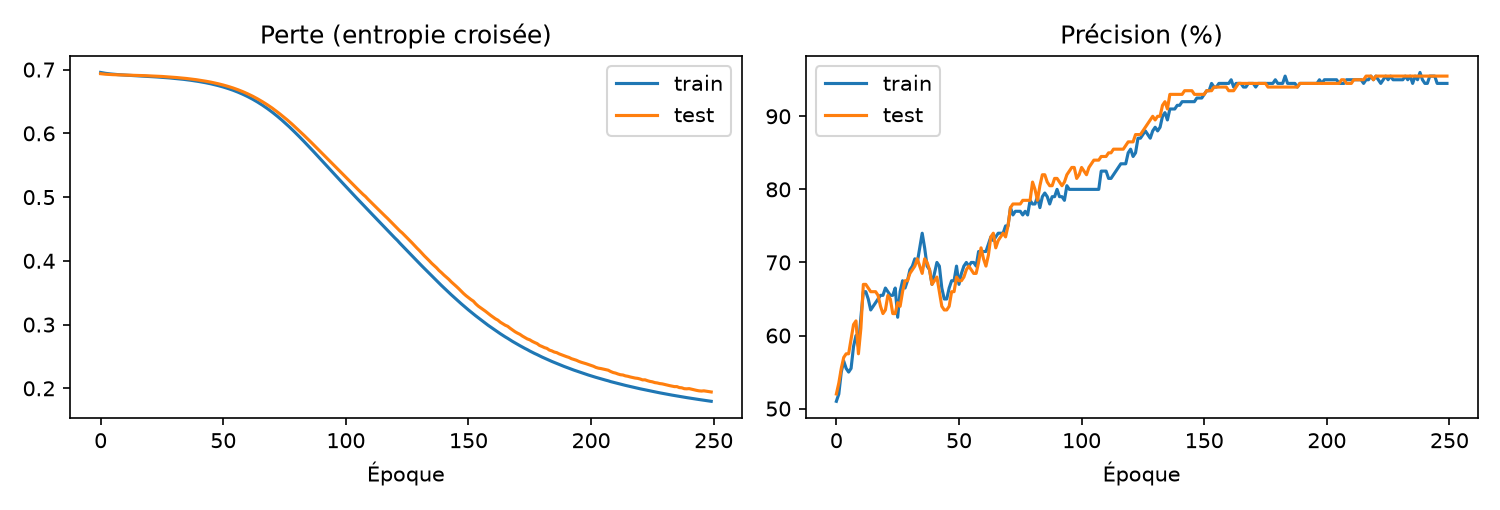
\includegraphics[width=0.78\textwidth]{figures/ab_reference.png}
\caption{Perte et précision sur \textit{Circles} ($\eta = 0.03$, batch 10, graine 0).}
\label{fig-ab_ref}
\end{figure}

\begin{figure}[H]
\centering
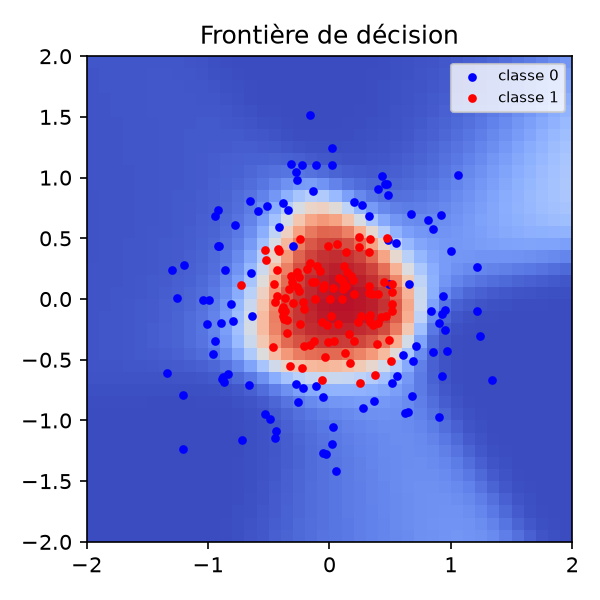
\includegraphics[width=0.36\textwidth]{figures/ab_frontiere.png}
\caption{Probabilité prédite pour la classe 1 sur la grille et points d'entraînement (même réseau qu'en \cref{fig-ab_ref}).}
\label{fig-ab_front}
\end{figure}

\subparagraph{Effet du pas d'apprentissage $\eta$ (batch 10).}
\begin{table}[H]
\centering
\small
\begin{tabular}{lccccccc}
\toprule
$\eta$ & $0.001$ & $0.01$ & $0.03$ & $0.1$ & $0.5$ & $2$ & $10$ \\
\midrule
Précision train & $60.3\%$ & $78.0\%$ & $95.7\%$ & $96.7\%$ & $96.5\%$ & $64.0\%$ & $71.2\%$ \\
Précision test & $60.7\%$ & $79.2\%$ & $\mathbf{95.0\%}$ & $94.2\%$ & $92.7\%$ & $63.0\%$ & $71.2\%$ \\
Écart-type test (3 graines) & $1.7$ & $2.7$ & $0.4$ & $1.0$ & $0.6$ & $18.4$ & $15.2$ \\
Époques pour $90\%$ en test & -- & -- & 116--155 & 39--48 & 11--17 & 20 / -- / -- & instable \\
\bottomrule
\end{tabular}
\end{table}

\begin{figure}[H]
\centering
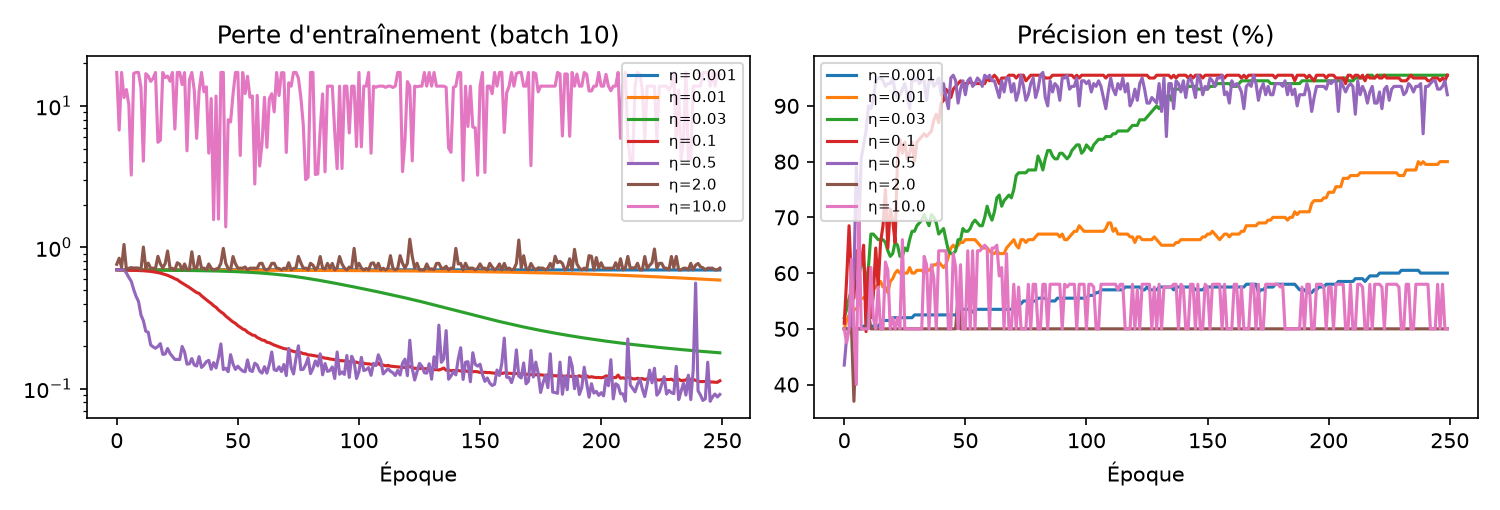
\includegraphics[width=0.9\textwidth]{figures/ab_learning_rate.png}
\caption{Perte d'entraînement (échelle logarithmique) et précision en test selon $\eta$ (batch 10, graine 0).}
\label{fig-ab_lr}
\end{figure}

Le pas d'apprentissage influence la convergence (\cref{fig-ab_lr}). Pour $\eta \leq 0.01$, le réseau se bloque sur le plateau initial et n'atteint jamais le seuil des $90\%$ de précision sur la durée des 250 époques. Entre $0.03$ et $0.5$, l'apprentissage converge d'autant plus rapidement que $\eta$ augmente : il faut environ 130 époques pour $\eta = 0.03$, 45 pour $\eta = 0.1$ et seulement 15 pour $\eta = 0.5$. Toutefois, un pas élevé rend l'évolution de la perte bruitée (pics apparaissant pour $\eta = 0.5$) et dégrade légèrement la précision en test ($92.7\%$). La perte d'entraînement descend plus bas ($0.09$) et le modèle commence à s'ajuster au bruit des données. Au-delà de cette plage, l'entraînement échoue. Avec $\eta = 2$, les premières mises à jour saturent les activations $\tanh$, ce qui laisse la perte autour de $0.69$ avec des performances très instables selon la seed ($63 \pm 18\%$). Enfin, pour $\eta = 10$, la saturation des sorties engendre des prédictions erronées mais plutôt confiantes : la perte dépasse alors 10 et la précision oscille entre $50\%$ et $65\%$.

\subparagraph{Effet de la taille de batch ($\eta = 0.03$).}
\begin{table}[H]
\centering
\small
\begin{tabular}{lcccc}
\toprule
Taille de batch & 1 (en ligne) & 10 & 50 & 200 (complet) \\
\midrule
Mises à jour en 250 époques & 50\,000 & 5\,000 & 1\,000 & 250 \\
Précision train & $96.8\%$ & $95.7\%$ & $70.2\%$ & $57.8\%$ \\
Précision test & $93.3\%$ & $\mathbf{95.0\%}$ & $67.7\%$ & $57.3\%$ \\
Époques pour $90\%$ en test & 14--19 & 116--155 & -- & -- \\
Temps total (CPU) & $10.5$\,s & $1.2$\,s & $0.35$\,s & $0.18$\,s \\
\bottomrule
\end{tabular}
\end{table}

\begin{figure}[H]
\centering
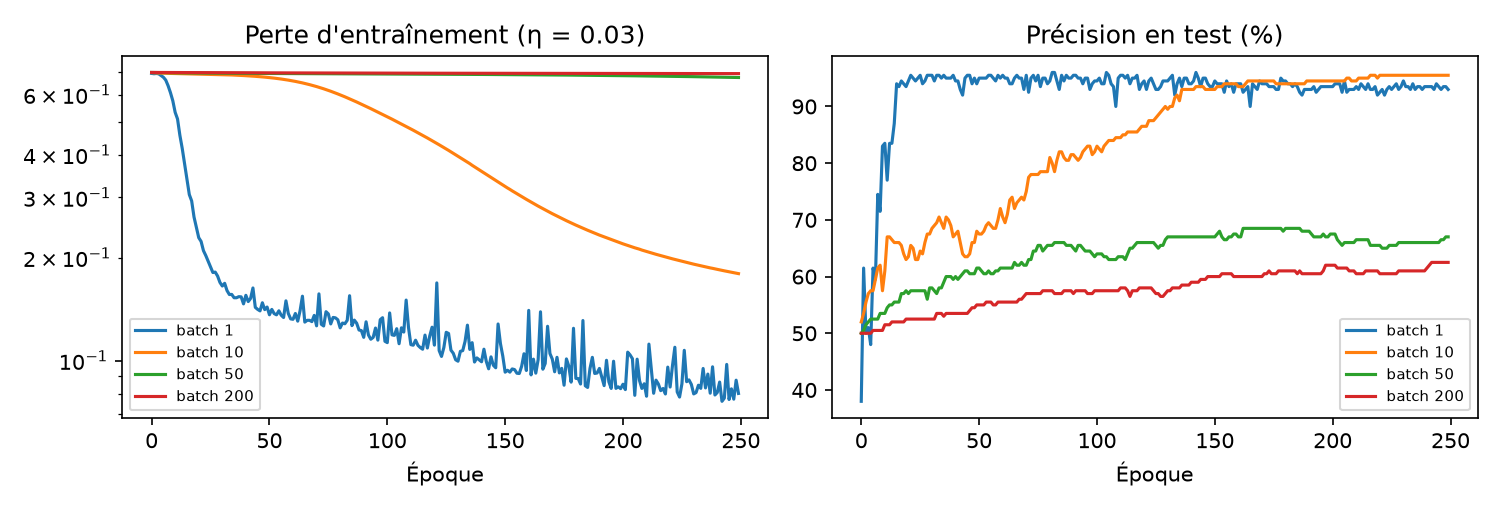
\includegraphics[width=0.9\textwidth]{figures/ab_batch_size.png}
\caption{Perte d'entraînement (échelle logarithmique) et précision en test selon la taille de batch ($\eta = 0.03$, graine 0).}
\label{fig-ab_bs}
\end{figure}

Comme nous faisons la moyenne de notre gradient sur chaque batch, l'augmentation de sa taille réduit le nombre total de mises à jour à $\eta$ et nombre d'époques constants. Avec le batch complet, le modèle n'effectue que 250 mises à jour et quitte à peine le plateau initial ($57\%$ de précision). À l'opposé, un batch de 1 converge le plus rapidement en nombre d'époques en atteignant jusqu'à $90\%$ dès la quinzième époque environ. Cependant, sa fonction de perte est très bruitée (\cref{fig-ab_bs}), il présente un léger surapprentissage ($96.8\%$ en entraînement contre $93.3\%$ en test), et l'absence de vectorisation le rend 9 fois plus lent qu'un batch de 10. Ce mini-batch de 10 réalise ainsi le meilleur compromis. Pour évaluer l'impact de la taille de batch, il serait intéressant d'ajuster $\eta$ proportionnellement ou de comparer les modèles dont le nombre de mises à jour est constant car ces deux hyperparamètres sont liés à un $\eta$ fixé.

\subsection{Simplifications avec \texttt{torch.autograd}, \texttt{torch.nn} et \texttt{torch.optim}}
\begin{itemize}
    \item \textbf{Partie 2 (\texttt{torch.autograd}) :} La fonction \texttt{backward()} manuelle disparaît. Les paramètres sont déclarés avec \texttt{requires\_grad=True}. L'appel \texttt{loss.backward()} applique la différentiation automatique sur le graphe dynamique. La mise à jour dans \texttt{sgd()} s'effectue sous \texttt{with torch.no\_grad():}.
    \item \textbf{Partie 3 (\texttt{torch.nn}) :} L'architecture est définie par \texttt{nn.Sequential(nn.Linear(nx, nh), nn.Tanh(), nn.Linear(nh, ny))}. La perte est calculée par \texttt{nn.CrossEntropyLoss()}, qui intègre en interne le $\text{LogSoftmax}$ stabilisé.
    \item \textbf{Partie 4 (\texttt{torch.optim}) :} L'optimiseur \texttt{optim.SGD(model.parameters(), lr=eta)} remplace la fonction \texttt{sgd()}. On utilise \texttt{optim.zero\_grad()} avant la rétropropagation et \texttt{optim.step()} après.
\end{itemize}
Après 150 itérations ($\eta = 0.03$), on obtient en test $96.0\%$ (autograd), $93.0\%$ (\texttt{torch.nn}) et $94.0\%$ (\texttt{torch.optim}), pour $94$ à $96\%$ en train. Ces trois versions sont mathématiquement équivalentes puisque les écarts de quelques points proviennent de l'initialisation aléatoire (aucune seed fixée) et de l'ordre des batchs.

\subsection{Application à MNIST}
Avec $n_x = 784$ ($28 \times 28$ pixels aplatis), $n_h = 100$, $n_y = 10$ classes, un batch de 100 et $\eta = 0.03$, le réseau atteint $86.4\%$ en test dès la première époque, puis plafonne autour de $89\%$ ($88.9\%$ en test et $88.6\%$ en train après 20 époques, avec un maximum de $90.6\%$ à l'époque 17), avec des oscillations de 1 à 2 points d'une époque à l'autre. Cette limite s'explique par l'absence de normalisation : les pixels sont dans $[0, 255]$, ce qui sature la fonction $\tanh$ de la couche cachée et rend le pas $\eta$ trop grand pour les poids d'entrée. Diviser les entrées par 255 (ou les standardiser) permettrait de dépasser nettement ce score. L'écart train/test est presque nul. Le modèle est limité par l'optimisation et non par le surapprentissage.

\subsection{Bonus : SVM}

\paragraph{Essayer d'abord un SVM linéaire (\texttt{LinearSVC}). Fonctionne-t-il bien ? Pourquoi ?}
Non : \texttt{LinearSVC} obtient $50.0\%$ en train et $53.0\%$ en test, soit le niveau du hasard (le \texttt{SVC} à noyau linéaire fait à peine mieux, $62\%$). Les données de \textit{Circles} étant constituées de deux cercles concentriques, aucun hyperplan (droite dans $\mathbb{R}^2$) ne peut les séparer.

\paragraph{Essayer ensuite des noyaux plus complexes (\texttt{SVC}). Lequel est le meilleur ? Pourquoi ?}
Résultats en test ($C = 1$) :
\begin{table}[H]
\centering
\small
\begin{tabular}{lccc}
\toprule
\textbf{Noyau} & \textbf{Train} & \textbf{Test} & \textbf{Vecteurs de support} \\
\midrule
Linéaire & $63.5\%$ & $62.0\%$ & 199 \\
Polynomial degré 2 & $95.5\%$ & $\mathbf{95.5\%}$ & 45 \\
Polynomial degré 3 & $57.5\%$ & $54.5\%$ & 192 \\
RBF & $96.0\%$ & $94.0\%$ & 55 \\
Sigmoïde & $57.5\%$ & $65.0\%$ & 143 \\
\bottomrule
\end{tabular}
\end{table}

Les noyaux polynomial de degré 2 et RBF obtiennent les meilleures performances. Le degré 2 est particulièrement adapté à la géométrie du problème : son espace de caractéristiques intègre directement les termes $x_1^2$ et $x_2^2$, de sorte que la frontière circulaire $x_1^2 + x_2^2 = r^2$ y devient linéaire (un hyperplan). Cela permet de séparer exactement les deux cercles concentriques avec peu de vecteurs de support. Le noyau RBF atteint un score comparable. En revanche, le noyau polynomial de degré 3 échoue car l'absence de terme constant ($(\gamma \langle x, x' \rangle)^3$) ne permet pas de générer les termes quadratiques purs nécessaires, alors que le noyau sigmoïde est inadapté pour modéliser une frontière de décision fermée.

\paragraph{Le paramètre de régularisation $C$ a-t-il un impact ? Pourquoi ?}
Oui, $C$ contrôle le compromis entre la largeur de la marge et la pénalité sur les erreurs. Avec le noyau RBF :
\begin{itemize}
    \item $C \leq 0.1$ : marge large, presque tous les points sont vecteurs de support (126 à 200) ; train $95.5\%$, test $95.0\%$. Les données étant peu bruitées, cette forte régularisation suffit.
    \item $C = 1$ : 55 vecteurs de support, train $96.0\%$, test $94.0\%$.
    \item $C \geq 10$ : 23 à 34 vecteurs de support, train jusqu'à $98.0\%$ mais test entre $93.0\%$ et $93.5\%$. La frontière s'ajuste aux points bruités : c'est le début du surapprentissage (\textit{overfitting}).
\end{itemize}
L'effet reste modéré sur ce jeu simple, mais il est possible d'observer que l'augmentation de $C$ améliore le train et dégrade légèrement le test.

\chapter{Réseaux de neurones convolutifs (1-cd)}

\section{Introduction aux réseaux convolutifs}

\paragraph{1. Pour un seul filtre de convolution de padding $p$, de stride $s$ et de taille de noyau $k$, et une entrée de taille $x \times y \times z$, quelle est la taille de sortie ? Combien y a-t-il de poids à apprendre ? Combien en faudrait-il pour une couche \textit{fully-connected} produisant une sortie de même taille ?}
 Pour une entrée $x \times y \times z$, un filtre de taille $k \times k$, un padding $p$ et un stride $s$ :
\begin{itemize}
    \item \textbf{Taille de sortie :} $x' \times y' \times 1$ avec $x' = \lfloor \frac{x + 2p - k}{s} \rfloor + 1$ et $y' = \lfloor \frac{y + 2p - k}{s} \rfloor + 1$.
    \item \textbf{Nombre de poids à apprendre :} $k \times k \times z$ (plus 1 biais, soit $k^2 z + 1$).
    \item \textbf{Couche dense équivalente :} Il faudrait $(x \cdot y \cdot z) \times (x' \cdot y')$ poids, ce qui est immensément plus élevé.
\end{itemize}

\paragraph{2. $\bigstar$ Quels sont les avantages de la convolution par rapport aux couches \textit{fully-connected} ? Quelle est sa principale limite ?}

\begin{itemize}
    \item \textbf{Avantages de la convolution :} Partage des poids (\textit{weight sharing}), équivariance par translation (un motif décalé dans l'image produit la même réponse, décalée d'autant, dans la carte de sortie ; l'invariance aux petites translations vient ensuite du \textit{pooling}, voir question 3), connectivité locale (\textit{sparse connectivity}) respectant la corrélation spatiale des pixels, et réduction massive du nombre de paramètres.
    \item \textbf{Principale limite :} Portée strictement locale des filtres ; impossibilité de capturer directement des relations globales distantes sans empiler de nombreuses couches.
\end{itemize}

\paragraph{3. $\bigstar$ Pourquoi utilise-t-on le \textit{pooling} spatial ?}
 Le pooling spatial sert à : (1) réduire la dimension spatiale et le coût calculatoire/mémoire ; (2) augmenter le champ récepteur des couches suivantes ; (3) apporter une invariance locale aux petites translations et distorsions.

\paragraph{4. $\bigstar$ Supposons qu'on calcule la sortie d'un réseau convolutif classique (par exemple VGG16) pour une image plus grande que la taille prévue ($224 \times 224$). Peut-on (sans modifier l'image) utiliser tout ou partie des couches du réseau sur cette image ?}
 \textbf{Oui}, toute la partie convolutive et pooling peut s'appliquer sans modification à une image plus grande (opérations locales glissantes). En revanche, les couches fully-connected exigent un vecteur d'entrée de dimension fixe ; pour les adapter, on remplace la mise à plat par un \textit{Global Average Pooling} (GAP) ou on convertit les couches denses en convolutions $1 \times 1$ (principe des réseaux FCN).

\paragraph{5. Si l'on ne s'intéresse qu'à un seul pixel de sortie, central, d'une convolution, comment modifier le filtre de convolution pour le rendre équivalent à une couche \textit{fully-connected} ?}
 Pour rendre le filtre équivalent à une couche dense sur un pixel central, on lui donne la taille exacte de l'entrée ($k_x = x, k_y = y$), avec $p=0$ et $s=1$. Le filtre couvre alors l'intégralité de l'image en une seule application, réalisant le produit scalaire complet.

\paragraph{6. Une convolution non partagée (\textit{unshared convolution}) conserve la connectivité locale des convolutions mais sans partage de poids. Pour une telle couche, avec une entrée de forme $(B, C, H, W)$ et $Q$ filtres de taille $5 \times 5$, combien de paramètres (hors biais) y a-t-il ?}
 Dans une convolution non partagée (\textit{unshared convolution}), chaque position spatiale de sortie possède ses propres poids. Pour une entrée $(B, C, H, W)$ et $Q$ filtres de taille $5 \times 5$ (sans padding, stride 1), la sortie spatiale est de taille $(H-4) \times (W-4)$. Le nombre de paramètres (hors biais) est :
\begin{equation}
    N = (H - 4)(W - 4) \times Q \times (5 \times 5 \times C) = 25 \cdot C \cdot Q \cdot (H - 4)(W - 4).
\end{equation}

\paragraph{7. On appelle champ récepteur d'un neurone l'ensemble des pixels de l'image dont dépend sa sortie. Quelle est la taille des champs récepteurs des neurones de la première et de la deuxième couche de convolution ? Que se passe-t-il pour les couches plus profondes ? Comment l'interpréter ?}
 Le champ récepteur $RF$ évolue selon $RF_l = RF_{l-1} + (k_l - 1) \cdot J_{l-1}$ où $J_{l-1} = \prod_{i=1}^{l-1} s_i$ :
\begin{itemize}
    \item \texttt{conv1} ($k=5, s=1$) : $RF = 5 \times 5$ pixels.
    \item \texttt{pool1} ($k=2, s=2$) : $RF = 5 + (2-1) \cdot 1 = 6 \times 6$ pixels (stride cumulé $J=2$).
    \item \texttt{conv2} ($k=5, s=1$) : $RF = 6 + (5-1) \cdot 2 = 14 \times 14$ pixels.
    \item Couches profondes : Après \texttt{pool2} ($J=4$) et \texttt{conv3} ($k=5$), $RF = 16 + 4 \cdot 4 = 32 \times 32$ pixels (toute l'image CIFAR-10).
    \item \textbf{Interprétation :} Les premières couches extraient des motifs locaux (bords, textures), tandis que les couches profondes intègrent ces motifs sur une large zone pour reconnaître des objets entiers.
\end{itemize}

\section{Entraînement \textit{from scratch} du modèle}
\subsection{Architecture du réseau}

\paragraph{8. Pour les convolutions, on veut conserver en sortie les mêmes dimensions spatiales qu'en entrée. Quelles valeurs de padding et de stride faut-il ?}
 Pour conserver la taille ($n' = n$) avec $s=1$, on résout $n + 2p - k + 1 = n \implies p = (k-1)/2$. Pour $k=5$, il faut $p=2$. Pour tout $k$ impair, $p$ est entier et centré ; pour $k$ pair, $k-1$ est impair, ce qui imposerait un padding asymétrique non isotrope.

\paragraph{9. Pour les \textit{max-poolings}, on veut diviser les dimensions spatiales par 2. Quelles valeurs de padding et de stride faut-il ?}
 Pour diviser la taille par 2 avec un max-pooling : fenêtre $k = 2$, stride $s = 2$, padding $p = 0$.

\paragraph{10. $\bigstar$ Pour chaque couche, indiquer la taille de sortie et le nombre de poids à apprendre. Commenter cette répartition.}
 Tableau des couches de \texttt{ConvNetCIFAR} ($3 \times 32 \times 32$) :
\begin{table}[H]
\centering
\small
\begin{tabular}{llccr}
\toprule
\textbf{Couche} & \textbf{Type} & \textbf{Sortie} & \textbf{Calcul des poids} & \textbf{Paramètres} \\
\midrule
\texttt{conv1} & Conv $5 \times 5$, pad 2 & $32 \times 32 \times 32$ & $(5 \times 5 \times 3 + 1) \times 32$ & 2\,432 \\
\texttt{pool1} & MaxPool $2 \times 2$, stride 2 & $32 \times 16 \times 16$ & Sans paramètre & 0 \\
\texttt{conv2} & Conv $5 \times 5$, pad 2 & $64 \times 16 \times 16$ & $(5 \times 5 \times 32 + 1) \times 64$ & 51\,264 \\
\texttt{pool2} & MaxPool $2 \times 2$, stride 2 & $64 \times 8 \times 8$ & Sans paramètre & 0 \\
\texttt{conv3} & Conv $5 \times 5$, pad 2 & $64 \times 8 \times 8$ & $(5 \times 5 \times 64 + 1) \times 64$ & 102\,464 \\
\texttt{pool3} & MaxPool $2 \times 2$ (\texttt{ceil}) & $64 \times 4 \times 4$ & Sans paramètre & 0 \\
\texttt{fc4}   & Dense vers 1000 & 1000 & $1024 \times 1000 + 1000$ & 1\,025\,000 \\
\texttt{fc5}   & Dense vers 10 & 10 & $1000 \times 10 + 10$ & 10\,010 \\
\midrule
\textbf{Total} & & & & \textbf{1\,191\,170} \\
\bottomrule
\end{tabular}
\end{table}

\textbf{Commentaire sur la répartition :} La couche dense \texttt{fc4} contient à elle seule $1\,025\,000$ paramètres, soit \textbf{$86\%$} du modèle, créant une vulnérabilité majeure au surapprentissage.

\paragraph{11. Quel est le nombre total de poids à apprendre ? Le comparer au nombre d'exemples.}
 Le total est de $1\,191\,170$ poids pour $50\,000$ images d'entraînement (environ 24 poids par image). Les degrés de liberté excédant largement les données, le risque de mémorisation est critique.

\paragraph{12. Comparer le nombre de paramètres à apprendre avec celui de l'approche BoW et SVM.}
 Dans l'approche BoW + SVM, les descripteurs (SIFT) sont fixes et le classifieur linéaire sur un vocabulaire de taille $K \approx 1000$ n'apprend que $10 \times K \approx 10\,000$ paramètres. Le CNN a beaucoup plus de paramètres car il apprend conjointement la représentation et la décision.

\subsection{Apprentissage du réseau}
\paragraph{13. Lire et tester le code fourni.}
 Le code fourni (LeNet-5~\cite{lecun1998} sur MNIST, SGD $\eta = 0.1$, batch 128) valide la boucle d'apprentissage : après 2 époques, on obtient $96.41\%$ en train et $97.40\%$ en test ($98.40\%$ et $98.44\%$ après 5 époques).

\paragraph{14. $\bigstar$ Dans le code fourni, quelle est la différence majeure entre la manière de calculer la perte et la précision en train et en test (en dehors de la différence de données) ?}
 En train, la perte et la précision sont calculées en moyenne glissante batch par batch pendant que les poids sont modifiés. En test, le modèle est figé en mode \texttt{eval()} et évalué de façon déterministe.

\paragraph{15. Modifier le code pour utiliser CIFAR-10 et implémenter l'architecture demandée. Faire assez d'époques pour que le modèle ait fini de converger.}
 Le code est adapté à CIFAR-10 (\texttt{datasets.CIFAR10}) avec l'architecture ci-dessus ; \texttt{count\_parameters} confirme les $1\,191\,170$ paramètres. Le modèle de base est entraîné 20 époques (SGD, $\eta = 0.1$, batch 128, environ 7\,s par époque sur GPU), durée suffisante puisque la précision en test plafonne dès l'époque 8 à 10.

\paragraph{16. $\bigstar$ Quels sont les effets du pas d'apprentissage et de la taille de batch ?}
 Toutes nos expériences utilisent $\eta = 0.1$ et un batch de 128 ; nous n'avons pas mené de balayage systématique de ces deux hyperparamètres. Leurs effets attendus sont les suivants. Le \textbf{learning rate} fixe l'amplitude des mises à jour : trop grand, la perte oscille ou diverge ; trop petit, la convergence est lente et peut s'arrêter dans un mauvais minimum. La \textbf{taille de batch} fixe la qualité de l'estimation du gradient : un grand batch donne un gradient moins bruité et exploite mieux le GPU (époques plus rapides), mais fait moins de mises à jour par époque et tend à généraliser un peu moins bien ; un petit batch apporte un bruit qui agit comme un régularisateur. Les deux sont liés : on augmente généralement $\eta$ avec la taille du batch.

\paragraph{17. Quelle est l'erreur au début de la première époque, en train et en test ? Comment l'interpréter ?}
 Au tout début de l'apprentissage, avec des poids aléatoires, le réseau prédit une distribution quasi uniforme : l'erreur est d'environ $90\%$ (précision $\approx 10\% = \frac{1}{10}$) et la perte vaut $-\ln(0.1) \approx 2.30$, en train comme en test. Les valeurs relevées à la fin de la première époque le confirment : en train, la précision moyenne sur l'époque est de $22.3\%$ pour une perte de $2.11$ ; en test, elle est de $36.6\%$ pour une perte de $1.76$. Le test est meilleur que le train car la métrique de train est une moyenne sur toute l'époque, qui inclut les premiers batchs prédits au hasard, alors que le test est évalué avec les poids de fin d'époque.

\paragraph{18. $\bigstar$ Interpréter les résultats. Qu'est-ce qui ne va pas ? Quel est ce phénomène ?}
 À l'issue des 20 époques du modèle de base : précision train $98.97\%$, précision test $68.81\%$. La précision en test plafonne entre $67\%$ et $70\%$ dès l'époque 8, et la perte de test atteint son minimum ($0.97$) à cette époque puis remonte jusqu'à $1.89$ (époque 19, $1.63$ à la fin), alors que la perte d'entraînement tend vers 0 ($0.04$). L'écart de $\approx 30$ points met en évidence un \textbf{surapprentissage massif} (\textit{overfitting}) : le réseau mémorise les exemples d'entraînement et devient de plus en plus confiant dans ses erreurs en test.

\section{Amélioration des résultats}

$\bigstar$ Pour chaque méthode mise en œuvre, nous indiquons en une phrase son principe et la raison pour laquelle elle améliore l'apprentissage.

\subsection{Standardisation des exemples}

\paragraph{19. Décrire vos résultats expérimentaux.}
 \textit{Principe :} on soustrait à chaque canal sa moyenne $\mu = [0.491, 0.482, 0.447]$ et on divise par son écart-type $\sigma = [0.202, 0.199, 0.201]$. \textit{Pourquoi cela aide :} les entrées sont centrées et à la même échelle, ce qui conditionne mieux le problème d'optimisation et accélère la convergence. \textit{Résultats :} pour gagner du temps, la standardisation a été évaluée conjointement avec l'augmentation de données (Run A, voir question 22) et non isolément. Son effet propre est visible au démarrage : en fin de première époque, la précision en train passe de $22.3\%$ (base) à $33.7\%$ (Run A), et en test de $36.6\%$ à $44.6\%$, signe d'une convergence plus rapide.

\paragraph{20. Pourquoi ne calculer l'image moyenne que sur les exemples d'entraînement, et normaliser les exemples de validation avec cette même image ?}
 Le jeu de test représente des données inconnues. Calculer les statistiques sur le test constituerait une \textbf{fuite d'information} (\textit{data leakage}).

\paragraph{21. Bonus : il existe d'autres schémas de normalisation, comme la normalisation ZCA. Essayer d'autres méthodes, expliquer les différences et les comparer à celle demandée.}
 Le blanchiment ZCA (\textit{Zero-phase Component Analysis}) décorrèle l'ensemble des pixels via les vecteurs propres de la covariance, éliminant les redondances tout en préservant la structure visuelle spatiale.

\subsection{Augmentation du nombre d'exemples par \textit{data augmentation}}
\paragraph{22. Décrire vos résultats expérimentaux et les comparer aux précédents.}
 \textit{Principe :} à chaque époque, chaque image d'entraînement est remplacée par une variante aléatoire (recadrage $28 \times 28$ et symétrie horizontale avec probabilité $1/2$, augmentations popularisées par AlexNet~\cite{krizhevsky2012}) ; en test, on applique un recadrage central $28 \times 28$. \textit{Pourquoi cela aide :} le réseau ne voit jamais deux fois exactement la même image, ce qui l'empêche de mémoriser et l'oblige à apprendre des caractéristiques invariantes à ces transformations. \textit{Résultats (Run A : standardisation + augmentation, 20 époques) :} précision train $86.68\%$, précision test \textbf{$78.97\%$} (contre $98.97\%$ / $68.81\%$ pour la base), soit $+10.2$ points en test et un écart train/test ramené de $30$ à $7.7$ points. La perte de test ne remonte plus : elle se stabilise vers $0.62$--$0.65$ (contre $1.63$). La précision en train est plus basse car la tâche d'entraînement est plus difficile, ce qui est attendu. Le coût est un temps par époque plus élevé ($\approx 16$\,s contre $7$\,s), dû aux transformations appliquées à la volée.

\paragraph{23. La symétrie horizontale semble-t-elle utilisable sur tous les types d'images ? Dans quels cas peut-elle l'être ou non ?}
 Valide pour les scènes naturelles et les objets symétriques ; totalement invalide pour les chiffres (MNIST : $6$ vs $9$), les lettres manuscrites (b vs d) ou les panneaux de signalisation routière.

\paragraph{24. Quelles limites voyez-vous à ce type d'augmentation de données par transformation du jeu de données ?}
 \begin{itemize}
    \item \textbf{Pas de nouvelle information :} les variantes sont des transformations d'images existantes. Elles n'apportent ni nouveaux objets, ni nouveaux points de vue, ni nouvelles conditions d'acquisition (éclairage, arrière-plan), et ne remplacent donc pas de vraies données supplémentaires.
    \item \textbf{Invariances choisies à la main :} chaque transformation impose une invariance que l'on suppose valide pour la tâche. Si elle ne l'est pas (symétrie pour les chiffres, question 23 ; rotation pour l'orientation d'une scène), l'augmentation introduit des exemples mal étiquetés.
    \item \textbf{Risque de dénaturer l'objet :} un recadrage trop agressif peut couper l'objet d'intérêt, de sorte que l'étiquette ne correspond plus au contenu visible.
    \item \textbf{Décalage train/test :} le réseau est entraîné sur des images transformées et évalué sur des images non transformées (recadrage central), ce qui crée un léger écart de distribution.
    \item \textbf{Coût :} les transformations appliquées à la volée sur CPU ralentissent l'entraînement (environ 16\,s contre 7\,s par époque dans nos runs) et la tâche plus difficile demande plus d'époques pour converger.
\end{itemize}

\paragraph{25. Bonus : d'autres méthodes d'augmentation de données sont possibles. Lesquelles ? En tester certaines.}
 Nous n'avons pas testé ces méthodes faute de temps ; nous décrivons les principales :
\begin{itemize}
    \item \textbf{Transformations photométriques} (\texttt{ColorJitter}) : variations aléatoires de luminosité, contraste, saturation et teinte, pour rendre le réseau robuste aux conditions d'éclairage.
    \item \textbf{Transformations géométriques supplémentaires} : petites rotations, translations, changements d'échelle (\texttt{RandomAffine}, \texttt{RandomResizedCrop}).
    \item \textbf{Cutout / Random Erasing} : masquage d'un rectangle aléatoire de l'image, qui force le réseau à utiliser plusieurs parties de l'objet plutôt qu'un seul indice discriminant.
    \item \textbf{Mixup} : combinaison convexe de deux images et de leurs étiquettes, $\tilde{x} = \lambda x_i + (1-\lambda) x_j$ et $\tilde{y} = \lambda y_i + (1-\lambda) y_j$ avec $\lambda \sim \text{Beta}(\alpha, \alpha)$. Cela lisse la frontière de décision et réduit la sur-confiance.
    \item \textbf{CutMix} : un rectangle d'une image est collé dans une autre, et les étiquettes sont mélangées au prorata de la surface. Il combine les avantages de Cutout et de Mixup.
    \item \textbf{Politiques apprises ou aléatoires} (AutoAugment, RandAugment) : application d'une séquence de transformations tirées dans une liste, avec une magnitude réglée par un ou deux hyperparamètres.
\end{itemize}
Sur CIFAR-10, Cutout, Mixup et CutMix apportent typiquement un à deux points de précision supplémentaires sur des réseaux plus profonds ; ils sont d'autant plus utiles que le modèle surapprend.

\subsection{Variantes de l'algorithme d'optimisation}
\paragraph{26. Décrire vos résultats expérimentaux et les comparer aux précédents, y compris en termes de stabilité de l'apprentissage.}
 \textit{Principe :} le pas décroît exponentiellement à chaque époque, $\eta_t = \eta_0 \cdot 0.95^t$, soit $\eta_{20} \approx 0.36\,\eta_0$ après 20 époques. \textit{Résultats :} nos runs A et B ont été entraînés à pas constant ($\eta = 0.1$) ; le scheduler n'a pas fait l'objet d'un run séparé, nous ne pouvons donc pas en chiffrer le gain. Ces runs montrent en revanche le problème qu'il vise : avec un pas constant, la précision en test oscille de plusieurs points d'une époque à l'autre (par exemple, dans le Run B, $76.8\%$, $73.9\%$, $70.6\%$ puis $79.1\%$ entre les époques 8 et 11, et encore de 1 à 2 points en fin d'entraînement). La décroissance du pas doit amortir ces oscillations et rendre la précision finale plus stable et légèrement meilleure.

\paragraph{27. Pourquoi cette méthode améliore-t-elle l'apprentissage ?}
 Un pas élevé permet de s'échapper rapidement des mauvais minima locaux au début, tandis qu'un pas réduit en fin d'entraînement permet d'atterrir précisément au fond de la cuvette d'optimisation.

\paragraph{28. Bonus : il existe de nombreuses autres variantes de SGD et stratégies de planification du pas d'apprentissage. Lesquelles ? En tester certaines.}
 Momentum de Polyak, Momentum de Nesterov, et méthodes à pas adaptatif : Adam, RMSprop et AdamW.

\subsection{Régularisation du réseau par \textit{dropout}}
\paragraph{29. Décrire vos résultats expérimentaux et les comparer aux précédents.}
 \textit{Principe :} le \textit{dropout}~\cite{srivastava2014}, ici \texttt{nn.Dropout(p=0.5)} entre \texttt{fc4} et \texttt{fc5} annule aléatoirement la moitié des activations de \texttt{fc4} à chaque passe d'entraînement. \textit{Pourquoi cela aide :} \texttt{fc4} concentre $86\%$ des paramètres ; le dropout l'empêche de mémoriser en forçant des représentations redondantes et robustes. \textit{Résultats :} le dropout a été évalué conjointement avec la batch normalization (Run B, en plus de la standardisation et de l'augmentation), et non isolément. Run B obtient $84.51\%$ en train et $81.78\%$ en test, contre $86.68\%$ / $78.97\%$ pour le Run A : la précision en train baisse (effet régularisant attendu) tandis que celle en test progresse de $2.8$ points, et l'écart train/test passe de $7.7$ à $2.7$ points. La perte de test descend à $0.53$ (contre $0.65$) et décroît encore à l'époque 20.

\paragraph{30. Qu'est-ce que la régularisation en général ?}
 Toute modification apportée à l'algorithme d'apprentissage visant à réduire l'erreur en test (généralisation) sans nécessairement réduire l'erreur d'entraînement.

\paragraph{31. Rechercher et discuter les interprétations possibles de l'effet du \textit{dropout} sur le comportement d'un réseau qui l'utilise.}
 Plusieurs interprétations complémentaires ont été proposées~\cite{srivastava2014} :
\begin{itemize}
    \item \textbf{Réduction de la co-adaptation :} un neurone ne peut pas compter sur la présence d'un autre neurone précis pour corriger ses erreurs. Chaque unité doit apprendre des caractéristiques utiles par elles-mêmes, ce qui donne des représentations plus redondantes et plus robustes.
    \item \textbf{Ensemble implicite :} chaque passe d'entraînement utilise un sous-réseau aminci différent parmi $2^N$ possibles ($N$ neurones concernés), tous partageant les mêmes poids. En test, utiliser le réseau complet avec des activations à l'échelle revient à approcher la moyenne (géométrique) des prédictions de cet ensemble, à un coût bien inférieur à l'entraînement de réseaux séparés.
    \item \textbf{Injection de bruit :} le dropout ajoute un bruit multiplicatif sur les activations, ce qui empêche le réseau de s'appuyer sur des configurations très précises des activations ; on peut le rapprocher de l'augmentation de données appliquée aux représentations internes.
    \item \textbf{Régularisation explicite :} pour un modèle linéaire, le dropout équivaut en espérance à une pénalité de type $L_2$ adaptative, pondérée par la variance de chaque entrée.
\end{itemize}
Dans notre réseau, ces effets se traduisent par une précision en train plus basse et un écart train/test réduit (question 29).

\paragraph{32. Quelle est l'influence de l'hyperparamètre de cette couche ?}
 Si $p=0$, aucune régularisation ; si $p$ est trop élevé ($> 0.7$), le réseau sous-apprend par manque de capacité de transmission du gradient. La valeur standard est $p=0.5$.

\paragraph{33. Quelle est la différence de comportement de la couche de \textit{dropout} entre l'entraînement et le test ?}
 En train, les activations sont masquées avec probabilité $p$ et divisées par $(1-p)$ (\textit{inverted dropout}) ; en test, la couche est désactivée (fonction identité).

\subsection{Utilisation de la \textit{batch normalization}}
\paragraph{34. Décrire vos résultats expérimentaux et les comparer aux précédents.}
 \textit{Principe :} après chaque convolution, une couche \texttt{BatchNorm2d}~\cite{ioffe2015} normalise chaque canal avec la moyenne et la variance du mini-batch, puis applique une transformation affine apprise. \textit{Pourquoi cela aide :} les distributions d'activations restent stables d'une couche à l'autre pendant l'apprentissage, ce qui autorise des pas plus grands et accélère la convergence. \textit{Résultats (Run B : standardisation + augmentation + BN + dropout) :} la convergence est nettement plus rapide : en fin de première époque, la précision est de $44.2\%$ en train et $46.7\%$ en test, contre $33.7\%$ / $44.6\%$ pour le Run A, et le Run B dépasse $70\%$ en test dès l'époque 4 (époque 6 pour le Run A). Après 20 époques, la précision en test atteint \textbf{$81.78\%$} (meilleur résultat de nos CNN), pour environ 16\,s par époque. Comme la perte de test diminue encore à la dernière époque, un entraînement plus long (éventuellement avec un scheduler) devrait encore améliorer ce score.

\chapter{CNN et introduction aux Vision Transformers (1-cde)}

\section{Partie 0 -- Échauffement : convolution et \textit{pooling}}

\paragraph{1. $\bigstar$ Pour un seul filtre de convolution de padding $p$, de stride $s$ et de taille de noyau $k$, et une entrée de taille $x \times y \times z$ : quelle est la taille de sortie ? Combien de poids faut-il apprendre ? Combien en faudrait-il pour une couche \textit{fully-connected} produisant une sortie de même taille ?}
Voir la question 1 du chapitre 1-cd.

\paragraph{2. $\bigstar$ Quels sont les avantages de la convolution par rapport aux couches \textit{fully-connected} ? Quelle est sa principale limite ?}
Voir la question 2 du chapitre 1-cd.

\paragraph{3. $\bigstar$ Pourquoi utilise-t-on le \textit{pooling} spatial ?}
Voir la question 3 du chapitre 1-cd.

\paragraph{4. $\bigstar$ Quel est le champ récepteur d'un neurone de \texttt{conv1}, puis de \texttt{conv2}, pour le réseau CIFAR-10 de la partie 1 ? Que se passe-t-il pour les couches plus profondes, et comment l'interpréter ?}
Voir la question 7 du chapitre 1-cd.

\paragraph{5. On donne à un CNN classique (par exemple VGG16, conçu pour des entrées $224 \times 224$) une image plus grande. Peut-on (sans modifier l'image) utiliser tout ou partie des couches du réseau ?}
Voir la question 4 du chapitre 1-cd.

\section{Partie 1 -- Entraînement d'un CNN \textit{from scratch}}

\paragraph{6. Lire et exécuter le code fourni (2 époques suffisent).}
Voir la question 13 du chapitre 1-cd.

\paragraph{7. $\bigstar$ Dans le code fourni, quelle est la différence majeure entre la manière de calculer la perte et la précision en train et en test (en dehors de la différence de données) ?}
Voir la question 14 du chapitre 1-cd.

\paragraph{8. $\bigstar$ Pour les convolutions, on veut une sortie de même taille spatiale que l'entrée. À partir de la formule de la question 1, déterminer le padding et le stride pour un noyau $5 \times 5$, puis pour un noyau de taille impaire $k$ quelconque. Pourquoi est-ce plus difficile avec un noyau de taille paire ? Pour les \textit{max-poolings}, on veut diviser la taille spatiale par 2 : quels padding et stride faut-il ?}
Voir les questions 8 et 9 du chapitre 1-cd.

\paragraph{9. $\bigstar$ Pour chaque couche, donner la taille de sortie et le nombre de poids à apprendre. Commenter cette répartition. Quel est le nombre total de poids ? Le comparer au nombre d'exemples d'entraînement.}
Voir les questions 10 et 11 du chapitre 1-cd.

\paragraph{10. Compléter \texttt{get\_dataset} pour CIFAR-10, implémenter le réseau et vérifier la réponse à la question 9 avec \texttt{count\_parameters}.}
\texttt{count\_parameters} donne bien $1\,191\,170$ paramètres. Voir la question 15 du chapitre 1-cd.

\paragraph{11. Entraîner le réseau (environ 20 époques). Quels sont les effets du pas d'apprentissage et de la taille de batch ?}
Voir la question 16 du chapitre 1-cd.

\paragraph{12. $\bigstar$ Quelle est l'erreur au début de la première époque, en train et en test ? Comment l'interpréter ?}
Voir la question 17 du chapitre 1-cd. (Le notebook ne comporte pas de question 13.)

\section{Partie 2 -- Amélioration du CNN}

\paragraph{14. Pourquoi \texttt{ceil\_mode=True} est-il nécessaire dans \texttt{pool3} une fois les images recadrées en $28 \times 28$ ?}
Avec des images recadrées à $28 \times 28$, la taille spatiale avant \texttt{pool3} est de $7 \times 7$. Sans \texttt{ceil\_mode}, la sortie spatiale serait $\lfloor 7/2 \rfloor = 3 \times 3$, donnant $64 \times 3 \times 3 = 576$ entrées, incompatible avec les 1024 neurones attendus par \texttt{fc4}. Avec \texttt{ceil\_mode=True}, la taille devient $\lceil 7/2 \rceil = 4 \times 4$, donnant exactement $64 \times 4 \times 4 = 1024$ entrées, préservant la compatibilité.

\paragraph{15. Décrire vos résultats et les comparer à la référence.}
Résultats du Run A (standardisation et augmentation) dans l'exécution du notebook 1-cde : la précision en test passe de $70.72\%$ à $77.46\%$ (train $87.06\%$). Voir les questions 19 et 22 du chapitre 1-cd pour l'analyse détaillée.

\paragraph{16. $\bigstar$ Pourquoi la moyenne et l'écart-type sont-ils calculés sur les seuls exemples d'entraînement, et aussi utilisés pour normaliser les exemples de test ?}
Voir la question 20 du chapitre 1-cd.

\paragraph{17. $\bigstar$ La symétrie horizontale semble-t-elle utilisable sur tous les types d'images ? Dans quels cas l'est-elle, ou non ?}
Voir la question 23 du chapitre 1-cd.

\paragraph{18. Décrire vos résultats et les comparer aux précédents.}
Résultats du Run B (\textit{batch normalization} et \textit{dropout} $0.5$) : la précision en test atteint $81.39\%$ (train $84.29\%$) et le surapprentissage est quasiment éliminé. Voir les questions 29 et 34 du chapitre 1-cd.

\paragraph{19. $\bigstar$ Ajouter un \textit{scheduler} du pas d'apprentissage (ou d'autres augmentations) et comparer.}
Voir la question 26 du chapitre 1-cd : le scheduler exponentiel ($\gamma = 0.95$) n'a pas fait l'objet d'un run séparé, son gain n'est donc pas chiffré. Les runs A et B à pas constant montrent les oscillations de plusieurs points en test qu'il vise à amortir.

\subsection{Tests en boîte noire : \textit{batch normalization} et \textit{dropout}}
\paragraph{20. $\bigstar$ Quelles implémentations sont correctes ? Pour chaque implémentation fautive, donner le test qui la met en défaut, la propriété vérifiée et le bug probable.}

\subparagraph{\textit{Batch normalization} mystère :}
\begin{itemize}
    \item \textbf{Couche A (Défaillante) :} Échoue au test d'indépendance en évaluation (\texttt{test\_bn\_eval\_independence} = False). Elle continue de normaliser avec les statistiques du mini-batch en mode \texttt{eval()} au lieu de geler et d'utiliser ses moyennes mobiles, violant l'indépendance des prédictions.
    \item \textbf{Couches B et C (Correctes) :} Valident l'ensemble des tests (conservation de taille, normalisation en train, indépendance en test).
\end{itemize}

\subparagraph{\textit{Dropout} mystère :}
\begin{itemize}
    \item \textbf{Couche A (Correcte) :} Valide la conservation de forme, l'identité en test et le rééchelonnage par $1/(1-p)$ en train.
    \item \textbf{Couche B (Défaillante) :} Échoue à \texttt{test\_dropout\_train\_scaling\_and\_masking}. Elle annule des neurones sans diviser par $1-p$, créant un déséquilibre d'amplitude entre train et test.
    \item \textbf{Couche C (Défaillante) :} Échoue à \texttt{test\_dropout\_eval\_identity}. Elle reste active en mode \texttt{eval()}, faussant les prédictions finales.
\end{itemize}

\section{Partie 3 -- Introduction aux Vision Transformers}

\subsection{\textit{Patch embedding}}
\paragraph{21. $\bigstar$ Implémenter le \textit{patch embedding} avec une seule \texttt{nn.Conv2d} traitant chaque patch $P \times P$ indépendamment, sans recouvrement (quels noyau et stride ?). Pourquoi est-ce exactement une projection linéaire des patchs aplatis ? Remettre ensuite le résultat sous la forme \texttt{(batch\_size, nb\_tokens, embed\_dim)}.}
On utilise \texttt{nn.Conv2d(in\_channels=3, out\_channels=D, kernel\_size=P, stride=P)}.
\begin{itemize}
    \item \textbf{Équivalence avec une projection linéaire :} Avec un noyau et un stride égaux à $P$, les fenêtres successives traitent des patchs disjoints de $P \times P$ pixels. Le produit de convolution sur chaque fenêtre calcule précisément le produit scalaire entre les $P^2 \times 3$ pixels aplatis et les poids de projection vers l'espace de dimension $D$.
    \item \textbf{Remodelage du tenseur :} On applique \texttt{x.flatten(2).transpose(1, 2)} pour transformer le tenseur de $(B, D, H/P, W/P)$ en $(B, N, D)$ où $N = (H/P)(W/P)$. Pour $28 \times 28$ avec $P=4$, $N = 7 \times 7 = 49$ tokens.
\end{itemize}

\subsection{Auto-attention}
\paragraph{22. $\bigstar$ Implémenter l'auto-attention à une tête.}
Pour $X \in \mathbb{R}^{N \times D}$, les Requêtes, Clés et Valeurs sont calculées par $Q = X W_Q$, $K = X W_K$, $V = X W_V$, puis :
\begin{equation}
    \text{Attention}(X) = \text{softmax}\left(\frac{Q K^\top}{\sqrt{D}}\right) V W_O.
\end{equation}

\paragraph{23. $\bigstar$ Quelle est la principale différence entre l'auto-attention et une convolution, en termes d'entrées dont dépend une sortie ? Quel est son principal coût en calcul et en mémoire ?}
\begin{itemize}
    \item \textbf{Dépendance des entrées :} La convolution est locale (voisinage fixe $k \times k$) avec des poids constants. L'auto-attention connecte tous les tokens entre eux de manière globale, avec des poids calculés dynamiquement selon la ressemblance du contenu.
    \item \textbf{Coût calculatoire et mémoire :} La convolution est en $\mathcal{O}(N \cdot k^2 D)$ (linéaire en nombre de pixels). L'auto-attention calcule la matrice $Q K^\top \in \mathbb{R}^{N \times N}$, induisant une complexité spatio-temporelle en $\mathcal{O}(N^2 D)$ (quadratique en nombre de tokens).
\end{itemize}

\subsection{Tests en boîte noire : auto-attention}
\paragraph{24. $\bigstar$ Quelles implémentations sont correctes ? Pour chaque implémentation fautive, donner le test qui échoue, la propriété vérifiée et le bug probable. Exécuter les mêmes tests sur notre \texttt{SelfAttention} et sur la \texttt{MultiHeadSelfAttention} fournie.}
Quels que soient ses poids, toute couche d'auto-attention correcte doit vérifier les propriétés suivantes. Les trois premières correspondent aux tests de base ; nous avons ajouté les deux dernières à partir de la question 23 (de quoi dépend un token de sortie ?) :
\begin{enumerate}
    \item \texttt{test\_attention\_shape} : la sortie a la même forme $(B, N, D)$ que l'entrée.
    \item \texttt{test\_attention\_batch\_independence} : la sortie d'une séquence ne dépend pas des autres séquences du batch. On compare la sortie de $x_1$ seul à celle de $x_1$ dans le batch $[x_1, x_2]$.
    \item \texttt{test\_attention\_permutation\_equivariance} : la couche ne contient aucune information de position, donc permuter les tokens d'entrée doit permuter la sortie de la même façon, $f(\Pi X) = \Pi f(X)$.
    \item \texttt{test\_attention\_global\_dependency} : l'attention est globale, donc modifier n'importe quel token $j$ doit modifier la sortie de tous les autres tokens $i \neq j$.
    \item \texttt{test\_attention\_uniform\_tokens} : si les $N$ tokens sont identiques, les poids d'attention sont uniformes et chaque sortie est égale à la sortie obtenue pour ce token seul.
\end{enumerate}

Notre \texttt{SelfAttention} et la \texttt{MultiHeadSelfAttention} fournie passent les cinq tests : aucun test ne rejette une couche correcte. Le module \texttt{mystery\_layers} n'étant compilé que pour Linux, les couches A à E ont été testées sur Colab (Python 3.13, PyTorch 2.14.1).

\begin{table}[H]
\centering
\footnotesize
\begin{tabular}{lccccc}
\toprule
\textbf{Couche} & \textbf{Forme} & \textbf{Indép. batch} & \textbf{Permutation} & \textbf{Dép. globale} & \textbf{Tokens identiques} \\
\midrule
A & True & True & \textbf{False} & \textbf{False} & True \\
B & True & True & True & True & True \\
C & True & True & \textbf{False} & \textbf{False} & \textbf{False} \\
D & True & \textbf{False} & True & True & True \\
E & True & True & True & True & True \\
\midrule
Notre \texttt{SelfAttention} & True & True & True & True & True \\
\texttt{MultiHeadSelfAttention} & True & True & True & True & True \\
\bottomrule
\end{tabular}
\end{table}

\textbf{B et E sont correctes} (au sens de ces tests). Pour localiser les bugs de A, C et D, nous avons calculé la matrice de dépendance $M_{ij} = 1$ si la sortie $i$ change quand on perturbe le token $j$ (séquence de 6 tokens) :
\begin{itemize}
    \item \textbf{A (fautive) :} échoue à l'équivariance par permutation et à la dépendance globale. Sa matrice de dépendance est \textbf{triangulaire inférieure} : le token $i$ ne dépend que des tokens $j \leq i$. Avec des tokens identiques, la sortie reste correcte, car seule la portée de l'attention change. Bug probable : un \textbf{masque causal} (celui des décodeurs de type GPT) appliqué à tort, alors qu'un encodeur ViT doit laisser chaque token voir tous les autres.
    \item \textbf{C (fautive) :} échoue à la permutation, à la dépendance globale et au test des tokens identiques. Sa matrice de dépendance est composée de blocs indépendants de 3 tokens, chaque token ne dépendant que de ses voisins immédiats, et des tokens identiques produisent des sorties qui varient avec la position. Ce motif s'explique exactement par un découpage erroné des têtes : \texttt{reshape(B, h, N, D/h)} appliqué directement au tenseur $(B, N, D)$, au lieu de \texttt{reshape(B, N, h, D/h).transpose(1, 2)}. Chaque « tête » reçoit alors des morceaux de canaux de tokens consécutifs au lieu d'une tranche de canaux de tous les tokens (avec $N = 6$, $D = 32$, $h = 4$ : la tête 0 couvre les tokens 0 et 1, la tête 1 les tokens 1 et 2, et ainsi de suite), ce qui reproduit la matrice observée.
    \item \textbf{D (fautive) :} échoue uniquement à l'indépendance du batch : la sortie de $x_1$ change de $0.42$ (écart maximal) quand on l'accompagne de $x_2$ dans le batch. Elle ne change pas si on l'accompagne d'une copie d'elle-même, ni si on passe 3 copies. Ce comportement correspond à une attention calculée sur les $B \times N$ tokens du batch aplatis en une seule séquence : chaque token voit aussi les tokens des autres images. Des clés et valeurs dupliquées ne modifiant pas une moyenne pondérée par softmax, les copies passent inaperçues. Bug probable : un \texttt{reshape(1, B*N, D)} (ou une multiplication matricielle sans dimension de batch) avant le calcul de $QK^\top$.
\end{itemize}

\textit{Limites :} ces tests vérifient des propriétés structurelles. Un softmax appliqué sur le mauvais axe, l'oubli du facteur $1/\sqrt{D}$ ou une inversion de $Q$ et $K$ les préservent tous, et ne seraient détectés qu'en comparant la couche à une implémentation de référence utilisant les mêmes poids. « Correcte » signifie donc ici : sans bug détectable par ces cinq propriétés.

\subsection{Le ViT complet}
\paragraph{25. Compléter le modèle ViT : un \textit{class token} appris, un plongement positionnel appris (un vecteur par token, [CLS] compris) et une tête linéaire appliquée au token [CLS] de sortie.}
Le modèle complet intègre le patch embedding, le token \texttt{[CLS]} apprenable concaténé en tête, l'addition des plongements positionnels, l'empilement des blocs Transformer (MultiHeadSelfAttention + MLP avec LayerNorm et résidus), et la tête linéaire branchée sur le token \texttt{[CLS]} de sortie.

\paragraph{26. $\bigstar$ Qu'est-ce que le token [CLS] et pourquoi l'utilise-t-on ? Pourquoi le plongement positionnel est-il nécessaire (que calculerait le réseau sans lui) ?}
\begin{itemize}
    \item \textbf{Token \texttt{[CLS]} :} Vecteur apprenable placé en tête de séquence, neutre spatialement. Il collecte l'information de l'ensemble de l'image par auto-attention et sert de descripteur global pour la classification, évitant un choix arbitraire de pooling spatial sur les patchs.
    \item \textbf{Plongements positionnels :} L'auto-attention étant purement équivariante par permutation, elle traite l'image comme un ensemble de patchs non ordonné (\textit{bag of tokens}). Sans plongements positionnels, une image dont les patchs sont mélangés de façon désordonnée donnerait exactement la même prédiction que l'image originale. Les plongements positionnels brisent cette symétrie et injectent la géométrie 2D.
\end{itemize}

\subsection{Entraînement}
\paragraph{27. Entraîner le ViT et le comparer aux CNN (nombre de paramètres, précision en test, écart train/test, temps d'entraînement par époque).}
Le ViT ($D = 128$, 4 blocs de 4 têtes, patchs $4 \times 4$, soit 49 tokens plus [CLS]) est entraîné 15 époques avec AdamW ($\eta = 10^{-3}$, \textit{weight decay} $0.05$), sur les mêmes données que le Run B (standardisation et augmentation, entrées $28 \times 28$). Les précisions ci-dessous viennent de l'exécution complète du notebook 1-cde ; elles diffèrent légèrement de celles du chapitre 1-cd, issues d'une autre exécution (initialisation aléatoire).

\begin{table}[H]
\centering
\small
\begin{tabular}{lcccccc}
\toprule
\textbf{Modèle} & \textbf{Paramètres} & \textbf{Époques} & \textbf{Train} & \textbf{Test} & \textbf{Écart} & \textbf{GPU/époque} \\
\midrule
CNN base & $1\,191\,170$ & 20 & $98.33\%$ & $70.72\%$ & $27.6$ & -- \\
CNN Run B & $1\,191\,490$ & 20 & $84.29\%$ & $\mathbf{81.39\%}$ & $2.9$ & $\approx 3.7$\,s \\
ViT & $807\,434$ & 15 & $74.35\%$ & $72.94\%$ & $1.4$ & $\approx 12.7$\,s \\
\bottomrule
\end{tabular}
\end{table}

\begin{itemize}
    \item \textbf{Paramètres :} le ViT compte $807\,434$ paramètres, soit $32\%$ de moins que le CNN ($1\,191\,490$ avec BN). Ils sont répartis sur les 4 blocs ($\approx 198\,000$ chacun, dont $\approx 132\,000$ pour le MLP), alors que $86\%$ des paramètres du CNN sont dans la seule couche \texttt{fc4}.
    \item \textbf{Précision en test :} $72.94\%$ pour le ViT, contre $81.39\%$ pour le CNN Run B, soit $8.5$ points de moins malgré des données et une boucle identiques. Le ViT fait mieux que le CNN de base ($70.72\%$), mais seulement grâce à la régularisation (augmentation et \textit{weight decay}).
    \item \textbf{Écart train/test :} faible pour les deux ($1.4$ point pour le ViT, $2.9$ pour le CNN). Le ViT ne surapprend pas : il \textbf{sous-apprend}. Sa précision en train n'est que de $74.35\%$ et progresse encore à la dernière époque, de même que la précision en test, et les deux pertes décroissent toujours. Plus d'époques amélioreraient donc son score, sans probablement rattraper le CNN.
    \item \textbf{Temps par époque :} mesuré sur la même carte (RTX 4080), le calcul pur d'une époque d'entraînement (391 batchs de 128) prend $\approx 12.7$\,s pour le ViT contre $\approx 3.7$\,s pour le CNN, soit $3.4$ fois plus, et le ViT utilise $3$ fois plus de mémoire GPU ($293$ contre $96$\,Mo). Les produits $QK^\top$ et les MLP sur 50 tokens dans chaque bloc coûtent plus cher que trois convolutions sur de petites cartes. Dans l'exécution complète du notebook (GPU Colab), l'écart est beaucoup plus faible ($\approx 18$\,s par époque pour le ViT contre $\approx 15$\,s pour le CNN), car le chargement et l'augmentation des images sur CPU représentent une grande part du temps.
    \item \textbf{Interprétation (biais inductifs contre besoin de données) :} le CNN possède des biais inductifs forts (localité, partage des poids, équivariance par translation) qui lui permettent d'apprendre efficacement sur $50\,000$ images. Le ViT n'en a presque aucun : chaque token peut interagir avec tous les autres dès la première couche, et la structure 2D n'est connue que via les plongements positionnels appris. Il doit donc apprendre ces régularités à partir des données, ce qui exige des volumes massifs (ImageNet-21k, JFT-300M) ou un pré-entraînement pour dépasser les CNN~\cite{dosovitskiy2021}.
\end{itemize}

\chapter*{Conclusion}
\addcontentsline{toc}{chapter}{Conclusion}

\noindent
Ces trois travaux pratiques ont permis de couvrir l'ensemble des fondements de la vision par apprentissage profond :
\begin{enumerate}
    \item La mise en œuvre manuelle sur \textit{Circles} et MNIST a permis d'illustrer le rôle central de la règle de dérivation en chaîne et l'efficacité des modules PyTorch pour automatiser l'optimisation.
    \item L'étude des CNN sur CIFAR-10 a illustré la puissance du partage des poids local tout en prouvant qu'un modèle profond est sujet au surapprentissage. Il est nécessaire de régulariser l'apprentissage (standardisation, augmentation, dropout, batch normalization).
    \item Enfin, l'introduction des Vision Transformers et la pratique des tests en boîte noire ont permis de mettre en application l'auto-attention globale.
\end{enumerate}

%%%%%%%%%%%%%%%%%%%%%%%%%%%%%%%%%%%%%%%%%%%%%%%%%%%%%%%%%%%%%%%%%%%%%%%%%%%%%%%
\begin{thebibliography}{9}
\bibitem{lecun1998} Y.~LeCun et al., \textit{Gradient-based learning applied to document recognition}, Proc. IEEE, 1998.
\bibitem{krizhevsky2012} A.~Krizhevsky et al., \textit{ImageNet classification with deep convolutional neural networks}, NeurIPS, 2012.
\bibitem{srivastava2014} N.~Srivastava et al., \textit{Dropout: a simple way to prevent neural networks from overfitting}, JMLR, 2014.
\bibitem{ioffe2015} S.~Ioffe, C.~Szegedy, \textit{Batch Normalization: Accelerating deep network training}, ICML, 2015.
\bibitem{dosovitskiy2021} A.~Dosovitskiy et al., \textit{An Image is Worth 16x16 Words: Transformers for Image Recognition at Scale}, ICLR, 2021.
\end{thebibliography}

\end{document}
